\documentclass[a4paper,11pt]{article}
\usepackage[margin=2cm]{geometry}
%\usepackage[utf8]{inputenc}
\usepackage{amsmath}
\usepackage{float}
\usepackage{stanli}
\usepackage{tikz}
\usetikzlibrary{arrows.meta,arrows,positioning}
\usepackage{ifthen}
\usepackage{adjustbox}
\usepackage[gobble=auto]{pythontex}
\usepackage[nameinlink]{cleveref}
\usepackage{graphicx}
\usepackage[absolute,overlay]{textpos}
\graphicspath{ {./images/Deffered/} }
% Differential
\newcommand*{\D}{\mathrm{d}}
% scientific notation
\providecommand{\e}[1]{\ensuremath{\times~10^{#1}}} 

\begin{pycode}
	import math
	def n(num, sig=3):
		f = '%.' + str(sig) + 'g' 
		ret = f % num
		if 'e' in ret:
			ret = ret.replace('e', r'\e{')
			ret += '}'
		return ret
	
	def to_eng(num, sig=3):
		try:
			x = int(math.log10(num)//3)*3
		except (ValueError, KeyError):
			x = 0
		if x != 0:
			ret = str(n(num/10**x,sig)) + r' \times 10^{' + str(x) + '}'
		else:
			ret = str(n(num,sig))
		return ret
\end{pycode}

% Commands for jinja2 templating
% Instead of empty braces (i.e. no command effect), here we make the variable uppercase red
% to emphasize in the template those variables to be replaced. Once rendered, this formatting
% has not effect as jinja replaces the \VAR{variable} entirely.
\usepackage{xcolor}
\newcommand*{\VAR}[1]{\textcolor{red}{\textbf{#1}}}
\newcommand*{\BLOCK}[1]{\textcolor{red}{\textbf{#1}}}

\usepackage{comment}
\newif\ifhidden
% This defines whether to show the hidden content or not.
\hiddenfalse 
\ifhidden 	% if \ hiddentrue
	\excludecomment{hidden}	% Exclude text within the "hidden" environment
\else   	% \ hiddenfalse
	\includecomment{hidden}		% Include text in the "hidden" environment
\fi

\title{CIV3221 Building structures and technology (Clayton and Sunway)\\
\VAR{FullName} (\VAR{StudentID})}
\date{Semester 2, 2020}
\usepackage{times}
\begin{document}
\maketitle
%\thispagestyle{fancy}

\begin{introduction}	
\noindent
\textbf{Introduction}\\
\noindent
This exam is an open-book assessment. The answers provided to all questions must be submitted through Moodle. You are allowed to use computational aid (including calculators), and to refer to lecture notes or other materials (that must be properly cited and referenced in order to avoid plagiarism).\\
\\ 
\noindent
Exam duration: 2 hours and 10 mins\\
\noindent
Scanning time: 30 mins\\

\end{introduction}
\begin{textblock*}{5cm}(8.9cm,28.49cm)
Page
\end{textblock*}
\begin{textblock*}{5cm}(10.1cm,28.49cm)
of 4
\end{textblock*}
%{\sf\tighttoc}
\newpage
\noindent
\textbf{QUESTION 1 [10 marks]}\\
a)	Identify differences between first and second order elastic analysis. \textbf{[5 marks]}\\
b)  What are the reasons that may cause the movement of facade. \textbf{[5 marks]}\\
\\
\begin{pycode}
	from testscript import *
	import random
	import math
	fn = open('read2.txt','r')
	for content in fn:
		iterator = int(content)
	fn.close()
	
	def allocation(aa, b):
		length = len(aa)
		product = []
		result = []
		fullproduct = 1
		for obj in aa:
			fullproduct = fullproduct * obj
		for i in range(1, length):
			product.append(1)
			for i in range(i, length):
				product[-1] = product[-1] * aa[i]
		r1= b%fullproduct
		for i in range(1, length):
			d1 = int(r1/product[i - 1])
			r1 = r1%product[i - 1]
			result.append(d1)
		result.append(r1)
		return result
	
	# ============================= Question 2 ============================
	para2_1 = [3, 3]
	al2_1 = allocation(para2_1, iterator)
	
	para2_2 = [3, 2]
	al2_2 = allocation(para2_2, iterator)
	
	para2_3 = [3, 3]
	al2_3 = allocation(para2_3, iterator)
		
	v21 = [10, 15, 20]
	v22 = [3, 4, 5]
	v23 = [10, 12, 15]
	v24 = [10.8, 21.6]
	v25 = [4, 6, 8]
	v26 = [4, 6, 8]
	
	sv21 = v21[al2_1[0]]
	sv22 = v22[al2_1[1]]
	sv23 = v23[al2_2[0]]
	sv24 = v24[al2_2[1]]
	sv25 = v25[al2_3[0]]
	sv26 = v26[al2_3[1]]
	
	# ============================= Question 3 ============================
	para3_1 = [3, 3, 2]
	para3_2 = [3, 3]
	para3_3 = [5, 3]
	al3_1 = allocation(para3_1, iterator)
	al3_2 = allocation(para3_2, iterator)
	al3_3 = allocation(para3_3, iterator)
	v31 = [3, 4, 5]
	v32 = [1, 2, 3]
	v33 = [32, 40]
	v34 = [2580, 2680, 2780]
	v35 = [120, 130, 140]
	v36 = [500, 600, 700, 800, 900]
	v37 = [1880, 1980, 2080]
	
	sv31 = v31[al3_1[0]]
	sv32 = v32[al3_1[1]]
	sv33 = v33[al3_1[2]]
	sv34 = v34[al3_2[0]]
	sv35 = v35[al3_2[1]]
	sv36 = v36[al3_3[0]]
	sv37 = v37[al3_3[1]]
	
	# ============================= Question 4 ============================
	para4_1 = [4, 3]
	al4_1 = allocation(para4_1, iterator)
	v41 = [7500, 7800, 8200, 8500]
	v42 = [1, 1.2, 1.5]
	
	sv41 = v41[al4_1[0]]
	sv42 = v42[al4_1[1]]
	
	# ============================= Question 5 ============================
	para5_1 = [3, 3, 3]
	al5_1 = allocation(para5_1, iterator)
	v51 = [1.0, 1.1, 1.2]
	v52 = [2000, 2200, 2500]
	v53 = [100, 120, 140]
	
	sv51 = v51[al5_1[0]]
	sv52 = v52[al5_1[1]]
	sv53 = v53[al5_1[2]]
	
	# ============================= Question 6 ============================
	para6 = [3, 4]
	al6 = allocation(para6, iterator)
	v61 = [400, 450, 500]
	v62 = [350, 400, 450]
	v63 = [1500, 1700, 1900, 2100]
	v64 = [1500, 1700, 1900, 2100]
	
	sv61 = v61[al6[0]]
	sv62 = v62[al6[0]]
	sv63 = v63[al6[1]]
	sv64 = v64[al6[1]]
	
	L_list = [3.5,3.75,4.0,4.25,4.5,4.75,5.0]  # m
	M_list = [-80, -30, -50]	# kNm
	I = 37.5e-6 	# m4
	J = 75e-6   	# m4
	E = 200     	# GPa
	G = 80      	# GPa
	
	# Unit conversions MNm2
	E *= 1e3
	G *= 1e3
	
	L = random.choice(L_list) 		# Member length
	M = random.choice(M_list) 		# y-axis moment load @ C
	
	grid = [L,I,J,E,G,M]
	
	EI_L = E*I/L
	GJ_L = G*J/L
	
	# Call analysis
	D = solve_D(grid)
	theta_C, theta_D, theta_F = D
	Fcd = eleF(eleK(grid),d_CD(D)*1e3)
	Fce = eleF(eleK(grid),d_CE(D)*1e3)
	Fcf = eleF(eleK(grid),d_CF(D)*1e3)
	Fgc = eleF(eleK(grid),d_GC(D)*1e3)
	Fcg = eleF(eleK(grid),d_CG(D)*1e3)
	
	bmd_scale=8
	tmd_scale=5
	
	iterator = iterator + 1
	fn = open('read2.txt','w')
	fn.write('%d' % iterator)
	fn.close()
\end{pycode}

\noindent
\textbf{QUESTION 2 [10 marks]}\\
For a continuous beam ABC shown in Figure Q2, the following loads are applied:\\
$\bullet$ External moment at Point A, M = $\py{sv21}$ kNm  anti-clockwise\\
$\bullet$ Uniformly distributed load (UDL) between Points A and B, w = $\py{sv22}$ kN/m \\
$\bullet$ Point load at midspan of BC, P = $\py{sv23}$ kN \\
Point A is free (unsupported), Support B is a roller and Support C is fixed.\\
Given: E = 200,000 MPa, I\textsubscript{AB} = 10.8 $\times$10$\textsuperscript{8}$mm$\textsuperscript{4}$, I\textsubscript{BC}=$\py{sv24}$ $\times$10$\textsuperscript{8}$mm$\textsuperscript{4}$, L\textsubscript{AB} = $\py{sv25}$ m, L\textsubscript{BC} = $\py{sv26}$ m\\
\begin{figure}[ht]
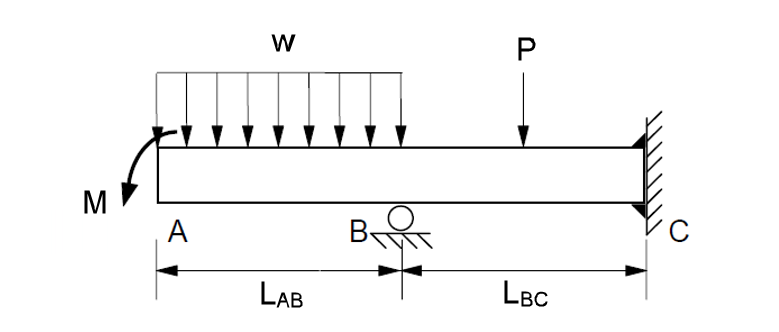
\includegraphics[width=9.53cm, height=4.37cm]{P2.png}\\
\centering
Figure Q2\\
\centering
\end{figure}
\\
a) Using the moment distribution method, calculate the support reactions at B and C. \textbf{[5 marks]}\\
b) Plot the bending moment and shear force diagrams. \textbf{[5 marks]}\\
\\
\\
\textbf{QUESTION 3 [20 marks]}\\
A simply supported composite slab in a composite floor structure of an office building is given below in Figure Q3. The live load is $\py{sv31}$ kPa. The dead load consists of the floor self-weight plus a super-imposed dead load of $\py{sv32}$ kPa . Take f'\textsubscript{c} = $\py{sv33}$ MPa , E\textsubscript{c} = 28000 MPa and unit weight of reinforced concrete = 25 kN/mm\textsuperscript{3} and L = $\py{sv34}$ mm.\\
\begin{figure}[ht]
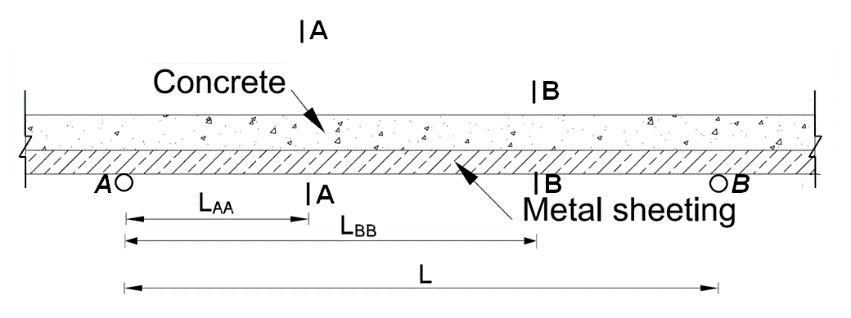
\includegraphics[width=11.08cm, height=4.16cm]{P3.png}\\
\centering
Figure Q3\\
\centering
\end{figure}
\\
a) Check the serviceability limit state condition of this span using the deemed-to-comply span to depth ratio method. Take the overall depth of slab D = $\py{sv35}$ mm. \textbf{[10 marks]}\\
b) What is the sagging bending moment capacity for the section A-A with a distance of L\textsubscript{A}\textsubscript{A} = $\py{sv36}$ mm  from the left support (A), and is it safe there in terms of bending moment capacity? \textbf{[5 marks]}\\
c) What is the sagging bending moment capacity for the section B-B with a distance of L\textsubscript{B}\textsubscript{B} = $\py{sv37}$ mm  from the left support (A), and is it safe there in terms of bending moment capacity? \textbf{[5 marks]}\\
\begin{textblock*}{5cm}(8.9cm,28.49cm)
Page
\end{textblock*}
\begin{textblock*}{5cm}(10.1cm,28.49cm)
of 4
\end{textblock*}
\newpage
\noindent
\textbf{QUESTION 4 [16 marks]}\\
The layout of a reinforced concrete floor is shown in Figure Q4 below for building construction. The overall depth of reinforced concrete slab is 120 mm. 460 UB 67.1 is used as the support steel girder for the secondary composite beam (nominal depth =460 mm, A\textsubscript{s} = 8580 mm\textsuperscript{2}, f\textsubscript{sy} = 300 MPa). All secondary beams are simply supported with a span length L of $\py{sv41}$  mm. The dead load consists of the floor self-weight plus a super-imposed dead load of $\py{sv42}$ kPa. Take f'\textsubscript{c} = 28 MPa, E\textsubscript{c} = 26,800 MPa and unit weight of reinforced concrete = 24 kN/m\textsuperscript{3}.\\
\\
a) What is the maximum live load that the composite beam can resist? \textbf{[8 marks]}\\
b) Calculate the number and spacing of welded shear studs that ensure complete shear connection. Use studs with d\textsubscript{bs} = 19 mm and f\textsubscript{uc} = 410 MPa. \textbf{[8 marks]}\\
\begin{figure}[ht]
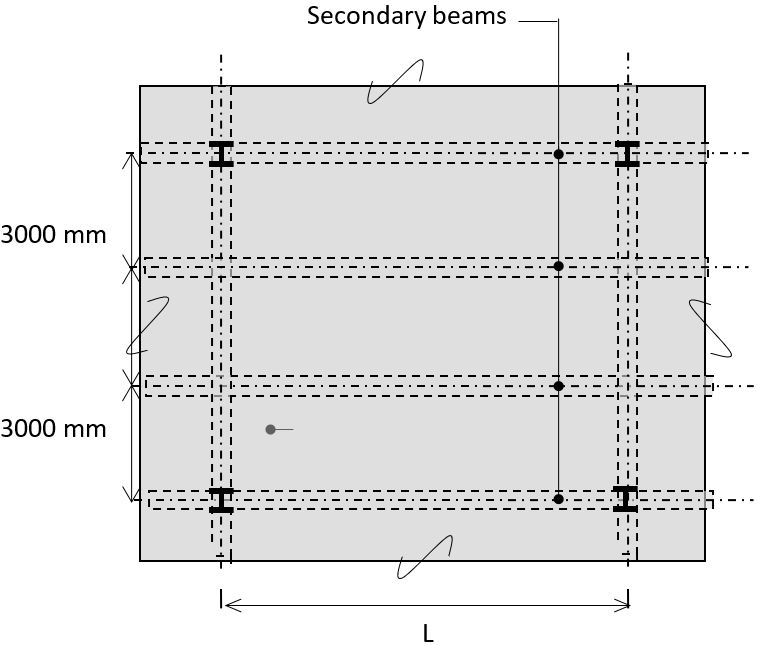
\includegraphics[width=10.47cm, height=9.39cm]{P4.png}\\
\centering
Figure Q4\\
\centering
\end{figure}
\\
\\
\\
\textbf{QUESTION 5 [30 marks]}\\
A 310UC158 (BHP 300 PLUS) is under combined compression force (N\textsuperscript{*}) and bending moment (M\textsubscript{x}\textsuperscript{*}) about its major x-axis. The capacity factor $\phi$ = 0.9. The moment ratio $\beta_m$ = $\py{sv51}$.\\
The applied compression force N\textsuperscript{*} is $\py{sv52}$ kN.  The bending moment M\textsubscript{x}\textsuperscript{*} is the product of N* and the load eccentricity (e) which is $\py{sv53}$ mm. The column length L = 3000 mm. The boundary condition of the column can be assumed as fixed at both ends. Section constant $\alpha_b$ = 0. Assume FLR is provided.\\
(a)	Calculate the design column member capacity about x-axis ($\phi$N\textsubscript{cx}). \textbf{[5 marks]}\\
(b)	Determine the design in-plane section and member capacities $\phi$M\textsubscript{rx} and $\phi$M\textsubscript{i} using the special formulae. Check if the member capacity is adequate. \textbf{[15 marks]}\\
(c)	Compare the maximum eccentricities (e) can be applied to the member for the given N\textsuperscript{*} based on the general and special formulae? \textbf{[10 marks]}\\
\\
\begin{textblock*}{5cm}(8.9cm,28.49cm)
Page
\end{textblock*}
\begin{textblock*}{5cm}(10.1cm,28.49cm)
of 4
\end{textblock*}
\newpage
\noindent
\textbf{QUESTION 6 [14 marks]}\\
Assuming that a typical column rests on a rectangular footing through a X\textsubscript{c}$\times$Y\textsubscript{c} ($\py{sv61}$$\times$$\py{sv62}$)  mm base plate, calculate the maximum design column load N\textsuperscript{*} the footing can support in terms of bending and punching shear. Assume planar dimensions of the footing to be X\textsubscript{b}$\times$Y\textsubscript{b} ($\py{sv63}$$\times$$\py{sv64}$) mm and its overall depth D = 500 mm with a concrete cover thickness of 75 mm. The concrete compressive strength f'\textsubscript{c} is 32 MPa and the steel reinforcements (f\textsubscript{y}=500 MPa) are placed as shown in Fig. Q6.\\
\begin{figure}[ht]
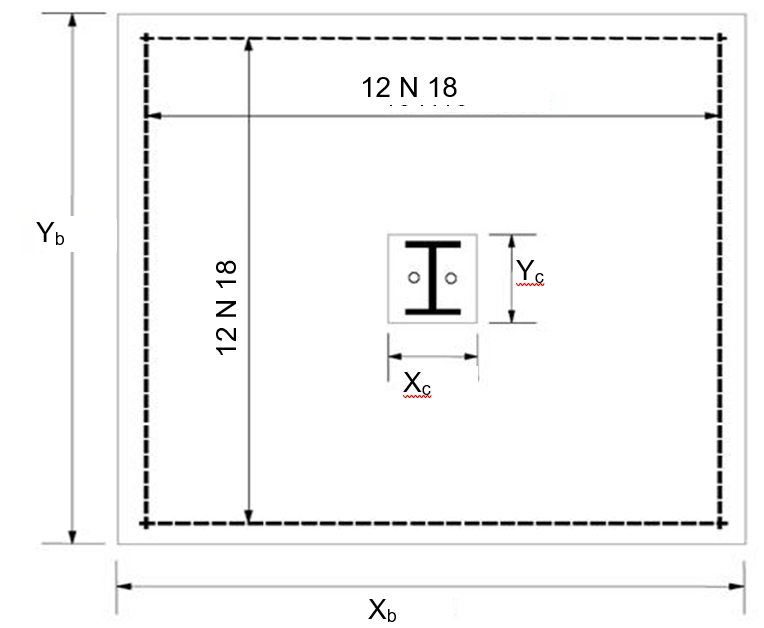
\includegraphics[width=8.94cm, height=8cm]{P6.png}\\
{\centering Figure Q6. Plan view of the footing for a single column (not to scale), with steel reinforcements N18 (diameter 18 mm) in each direction\par}\\
\end{figure}
\\
\\
\\
\\
\\
\\
\\
\\
\\
\\
\begin{figure}[ht]
\centering{\textbf{End of exam paper}}\par\\
\end{figure}
\begin{textblock*}{5cm}(8.9cm,28.49cm)
Page
\end{textblock*}
\begin{textblock*}{5cm}(10.1cm,28.49cm)
of 4
\end{textblock*}
\begin{hidden}	
\clearpage
\section{Solution}

\textbf{Step 1:} Define coordinate system. This is already provided in \Cref{fig:grid}. 

\textbf{Step 2:} The unknown degrees of freedom are: 

\begin{itemize}
	\item Rotation about global y-axis at C ($\theta_C$)
	\item Rotation about global y-axis at D ($\theta_D$)
	\item Rotation about global y-axis at F ($\theta_F$)
\end{itemize} 

Due to symmetry of members CD and CF, and no applied point load, the degree of freedom for translation C is known: $\delta_C = 0$. Hence; 

\begin{equation}
	DOF = \left\{\theta_C,\theta_D,\theta_F\right\}
\end{equation}

\textbf{Step 3:} The known forces corresponding to the unknown DOF are: 

\begin{equation}
	F = \left\{ \py{n(M)},0,0 \right\} \textrm{\hspace{0.5cm} [kNm]}
\end{equation}

Note, the negative sign as per the direction of the double-headed arrow. 
	
\textbf{Step 4:} Apply $\theta_C$ positively only. 

This causes bending along member DCF, and twisting along member ECG. 

\textbf{Step 5:} Get forces at each DOF. 

Moment in the direction of $\theta_C$ caused by $\theta_C$: 

\begin{itemize}
	\item In Element DC: $M_C = \left(\frac{4EI}{L}\right)\theta_C$
	\item In Element CF: $M_C = \left(\frac{4EI}{L}\right)\theta_C$
	\item In Element EC: $M_C = \left(\frac{GJ}{L}\right)\theta_C$
	\item In Element CG: $M_C = \left(\frac{GJ}{L}\right)\theta_C$
\end{itemize}	

As all member properties are equal, then: 

\begin{equation}
	M_C = \frac{8EI+2GJ}{L}\theta_C
\end{equation}

Moment in the direction of $\theta_D$ caused by $\theta_C$: 

\begin{itemize}
	\item In Element DC: $M_D = \left(\frac{2EI}{L}\right)\theta_C$
\end{itemize}	

Moment in the direction of $\theta_F$ caused by $\theta_C$: 

\begin{itemize}
	\item In Element CF: $M_F = \left(\frac{2EI}{L}\right)\theta_C$
\end{itemize}	

\textbf{Step 6:} Repeat for each DOF

Apply $\theta_D$ positively only and get forces at each DOF. 

Moment in the direction of $\theta_C$ caused by $\theta_D$: 

\begin{itemize}
	\item In Element DC: $M_C = \left(\frac{2EI}{L}\right)\theta_D$
\end{itemize}	

Moment in the direction of $\theta_D$ caused by $\theta_D$: 

\begin{itemize}
	\item In Element DC: $M_D = \left(\frac{4EI}{L}\right)\theta_D$
\end{itemize}	

Moment in the direction of $\theta_F$ caused by $\theta_D$ is equal to zero ($M_F = 0$) as there is no rotation (C is locked).

Apply $\theta_F$ positively only and get forces at each DOF. 

Moment in the direction of $\theta_C$ caused by $\theta_F$: 

\begin{itemize}
	\item In Element DC: $M_C = \left(\frac{2EI}{L}\right)\theta_F$
\end{itemize}	

Moment in the direction of $\theta_D$ caused by $\theta_F$ is equal to zero ($M_D = 0$) as there is no rotation (C is locked).		

Moment in the direction of $\theta_F$ caused by $\theta_F$: 

\begin{itemize}
	\item In Element DC: $M_F = \left(\frac{4EI}{L}\right)\theta_F$
\end{itemize}			
		
\textbf{Step 7:} Add nodal forces

Total moment in the direction of $\theta_C$: 

\begin{equation}
	M_C = \frac{8EI+2GJ}{L}\theta_C +  \left(\frac{2EI}{L}\right)\theta_D + \left(\frac{2EI}{L}\right)\theta_F  
\end{equation}

Total moment in the direction of $\theta_D$: 

\begin{equation}
	M_D = \left(\frac{2EI}{L}\right)\theta_C + \left(\frac{4EI}{L}\right)\theta_D + 0  
\end{equation}

Total moment in the direction of $\theta_F$:

\begin{equation}
	M_F = \left(\frac{2EI}{L}\right)\theta_C + 0 \left(\frac{4EI}{L}\right)\theta_F  
\end{equation}

Given: 

\begin{equation}
\frac{EI}{L} = \frac{ \left( \py{to_eng(E)} \right)\left(\py{to_eng(I)}\right) }
					{ \left(\py{to_eng(L)}\right) } \times 10^{-3}
				=\py{to_eng(EI_L*1e3)}~\mathrm{kNm}
\end{equation}


\begin{equation}
\frac{GJ}{L} = \frac{ \left( \py{to_eng(G)} \right)\left(\py{to_eng(J)}\right) }
					{ \left(\py{to_eng(L)}\right) } \times 10^{-3}
				=\py{to_eng(GJ_L*1e3)}~\mathrm{kNm}
\end{equation}

The resulting structural stiffness matrix becomes: 

\begin{equation}
	K = 10^3 \py{m2ltx(sysK(grid))}
\end{equation}

Notice, it is symmetrical, giving confidence we have done it correctly.  

\textbf{Step 8:} Solve, using Rule of Sarrus and Cramer's Rule to find:
	
\begin{align*}
	\begin{Bmatrix}
		\theta_C \\ \theta_D \\ \theta_F
	\end{Bmatrix} 
	&= 10^{-3} 
	{\py{m2ltx(sysK(grid))}}^{-1}
	\py{m2ltx(getF(grid),style='Bmatrix')} \\
	&= \frac{10^{-3}}{\py{to_eng(det_K(sysK(grid)))}} \py{m2ltx(inv_K(sysK(grid))*det_K(sysK(grid)))}
	\py{m2ltx(getF(grid),style='Bmatrix')} \\
\end{align*}
from which:
\begin{equation}
	\begin{Bmatrix}
		\theta_C \\ \theta_D \\ \theta_F
	\end{Bmatrix} 
	= \py{m2ltx(D*1e3,style='Bmatrix')}	~\mathrm{[mrad]}
\end{equation}

\textbf{Step 9:} Member forces:

Using the special matrix since there is no vertical force and no
vertical displacement for this special case.

For Member \emph{CD}:
\begin{equation*}
	\begin{Bmatrix}
	T_C \\ M_C \\ T_D \\ M_D
	\end{Bmatrix} 
	= 10^{3} 
	\py{m2ltx(eleK(grid))}
	\py{m2ltx(d_CD(D*1e3),style='Bmatrix')}
	= 
	\py{m2ltx(Fcd,style='Bmatrix')}
	~\mathrm{[kNm]}
\end{equation*}

For Member \emph{CF} we consider not using the lower number node as the $i$ node to illustrate the coordinate transform that must be considered. In this case, since the local $z$-axis and gloabl $Y$-axis are parallel, positive $\theta$ become positive major axis bending in the member's local coordinate system:

\begin{equation*}
	\begin{Bmatrix}
		T_C \\ M_C \\ T_F \\ M_F
	\end{Bmatrix} 
	= 10^{3} 
	\py{m2ltx(eleK(grid))}
	\py{m2ltx(d_FC(D*1e3),style='Bmatrix')}
	= 
	\py{m2ltx(Fcf,style='Bmatrix')}
	~\mathrm{[kNm]}
\end{equation*}


For Member \emph{CE}:
\begin{equation*}
	\begin{Bmatrix}
		T_C \\ M_C \\ T_E \\ M_E
	\end{Bmatrix} 
	= 10^{3} 
	\py{m2ltx(eleK(grid))}
	\py{m2ltx(d_CE(D*1e3),style='Bmatrix')}
	= 
	\py{m2ltx(Fce,style='Bmatrix')}
	~\mathrm{[kNm]}
\end{equation*}

And finally, for Member \emph{CG}, we again break convention and carefully consider the directions of the global displacements as they relate to the local member coordinate system.

\begin{equation*}
	\begin{Bmatrix}
		T_G \\ M_G \\ T_C \\ M_C
	\end{Bmatrix} 
	= 10^{3} 
	\py{m2ltx(eleK(grid))}
	\py{m2ltx(d_GC(D*1e3),style='Bmatrix')}
	= 
	\py{m2ltx(Fgc,style='Bmatrix')}
	~\mathrm{[kNm]}
\end{equation*}

\textbf{Step 10} is to draw the internal actions diagrams. To do this, the results of the member actions which were derived in the local member coordinate system must now be considered now in the global coordinate system. The easiest way to do this is to draw the directions by carefully interpreting the member force signs against the global axis system. The resulting FBD is shown in \Cref{fig:fbd}.

\begin{figure}[!htb]
	\centering
	
	\begin{pysub}
		\setcoords{-25}{30}[1][1] 
		\setaxis{2} 
		\begin{adjustbox}{max width=\textwidth}
			\begin{tikzpicture}[coords] 
			\dscaling{1}{1.5};
			
			\dpoint{c}{0}{0}{0}; 
			\dpoint{d}{ -!{L} }{0}{0};
			\dpoint{e}{0}{ !{L} }{0}; 
			\dpoint{f}{ !{L} }{0}{0};
			\dpoint{g}{0}{-!{L} }{0}; 
			\dpoint{z}{ -!{0.7*L} }{ -!{0.7*L} }{0}; 
			
			\daxis{1}{z}; 
			
			\dbeam{1}{c}{d};
			\dbeam{1}{c}{e};
			\dbeam{1}{c}{f};
			\dbeam{1}{c}{g};
			
			\support{1}{d}; \hinge{1}{d}
			\support{3}{e}[90];
			\support{1}{f}; \hinge{1}{f}
			\support{3}{g}[270];

			\begin{scope}[force/.append style={color=red,>={Latex[length=0pt 5]}},
			normalLine/.append style={line width=1mm}]
				
				\dload{4}{c}[90][-90][ !{L/3} ];
				\dnotation{1}{c}{$!{n(abs(Fcg[0]))}$}[left=5mm];

				\dload{3}{c}[270][-90][ !{L/3} ];
				\dnotation{1}{c}{$!{n(abs(Fce[0]))}$}[right=5mm];				
				
				\dpoint{cd}{-!{L/6}}{0}{0}
				\dload{4}{cd}[90][-90][ !{L/3} ];
				\dnotation{1}{cd}{$!{n(abs(Fcd[1]))}$}[left=5mm];

				\dpoint{cf}{!{L/6}}{0}{0}
				\dload{4}{cf}[90][-90][ !{L/3} ];
				\dnotation{1}{cf}{$!{n(abs(Fcf[1]))}$}[below=5mm];
				
				\dload{4}{g}[270][-90][ !{L/3} ];
				\dnotation{1}{g}{$!{n(abs(Fcg[2]))}$}[right=5mm];

				\dload{3}{e}[90][-90][ !{L/3} ];
				\dnotation{1}{e}{$!{n(abs(Fce[2]))}$}[left=5mm];	
				
			\end{scope}
			
			\dnotation{1}{c}{$C$}[above=2mm];
			\dnotation{1}{d}{$D$}[above right];
			\dnotation{1}{e}{$E$}[above left];
			\dnotation{1}{f}{$F$}[above right];
			\dnotation{1}{g}{$G$}[below right];
			
			\end{tikzpicture}
		\end{adjustbox}
	\end{pysub}
	\caption{Free body diagram.}
	\label{fig:fbd}
\end{figure}

Considering the BMD, for each member, to identify the side in tension it can help to visualise the deformation resulting from the forces acting on it indicated in the free body diagram, \Cref{fig:fbd}. Since there are no loads acting between the nodes, the BMD is comprised of straight lines between the values at each node. The BMD is shown in \Cref{fig:bmd}.

\begin{figure}[ht]
	\centering
	
	\begin{pysub}
		\setcoords{-25}{30}[1][1][1] 
		\setaxis{2} 
		\begin{adjustbox}{max width=\textwidth}
			\begin{tikzpicture}[coords] 
			\dscaling{1}{1.5};
			
			\dpoint{c}{0}{0}{0}; 
			\dpoint{d}{ -!{L} }{0}{0};
			\dpoint{e}{0}{ !{L} }{0}; 
			\dpoint{f}{ !{L} }{0}{0};
			\dpoint{g}{0}{-!{L} }{0}; 
			\dpoint{z}{ -!{0.7*L} }{ -!{0.7*L} }{0}; 
			
			\daxis{1}{z}; 
			
			\dbeam{1}{c}{d};
			\dbeam{1}{c}{e};
			\dbeam{1}{c}{f};
			\dbeam{1}{c}{g};
			
			\support{1}{d};  \hinge{1}{d}
			\support{3}{e}[90];
			\support{1}{f};  \hinge{1}{f}
			\support{3}{g}[270];
			
			\dinternalforces{xz}{c}{d}{ !{int(Fcd[1]/bmd_scale)} }{ !{int(Fcd[3]/bmd_scale)} };
			\dinternalforces{xz}{c}{e}{ !{int(Fce[1]/bmd_scale)} }{ !{int(Fce[3]/bmd_scale)} };
			\dinternalforces{xz}{c}{f}{ !{int(Fcf[1]/bmd_scale)} }{ !{int(Fcf[3]/bmd_scale)} };
			\dinternalforces{xz}{c}{g}{ !{int(Fcg[1]/bmd_scale)} }{ !{int(Fcg[3]/bmd_scale)} };
			
			\dnotation{1}{c}{$!{n(abs(Fcd[1]))}$}[below right=18mm and 0mm of c];
			\dnotation{1}{c}{$!{n(abs(Fcf[1]))}$}[above left=18mm and 0mm of c];
			
			\dnotation{1}{c}{$C$}[right=3mm];
			\dnotation{1}{d}{$D$}[above right];
			\dnotation{1}{e}{$E$}[above left];
			\dnotation{1}{f}{$F$}[above right];
			\dnotation{1}{g}{$G$}[below right];
			
			\end{tikzpicture}
		\end{adjustbox}
	\end{pysub}
	\caption{Bending Moment Diagram.}
	\label{fig:bmd}
\end{figure}

For the TMD, it is not necessary to adopt a strict drawing convention once the relative actions are indicated. For example, the double-headed arrow in \Cref{fig:fbd} indicating the torsion of member $CE$ could be thought of as an analogous ``tension'' which we may consider as positive, and so we draw the TMD above the line. Similarly, fr member $CG$, the double-headed arrows act in the opposite sense to the analogous ``tension'' and so are analogous to ``compression'', which we then draw on the bottom of the member, as shown in \Cref{fig:tmd}.

\begin{figure}[ht]
	\centering
	
	\begin{pysub}
		\setcoords{-25}{30}[1][1][1] 
		\setaxis{2} 
		\begin{adjustbox}{max width=\textwidth}
			\begin{tikzpicture}[coords] 
			\dscaling{1}{1.5};
			
			\dpoint{c}{0}{0}{0}; 
			\dpoint{d}{ -!{L} }{0}{0};
			\dpoint{e}{0}{ !{L} }{0}; 
			\dpoint{f}{ !{L} }{0}{0};
			\dpoint{g}{0}{-!{L} }{0}; 
			\dpoint{z}{ -!{0.7*L} }{ -!{0.7*L} }{0}; 
			
			\daxis{1}{z}; 
			
			\dbeam{1}{c}{d};
			\dbeam{1}{c}{e};
			\dbeam{1}{c}{f};
			\dbeam{1}{c}{g};
			
			\support{1}{d};  \hinge{1}{d}
			\support{3}{e}[90];
			\support{1}{f};  \hinge{1}{f}
			\support{3}{g}[270];
			
			\dinternalforces{yz}{c}{d}{ !{int(Fcd[0]/tmd_scale)} }{ !{int(-Fcd[2]/tmd_scale)} };
			\dinternalforces{yz}{c}{e}{ !{int(Fce[0]/tmd_scale)} }{ !{int(-Fce[2]/tmd_scale)} };
			\dinternalforces{yz}{c}{f}{ !{int(Fcf[0]/tmd_scale)} }{ !{int(-Fcf[2]/tmd_scale)} };
			\dinternalforces{yz}{c}{g}{ !{int(Fcg[0]/tmd_scale)} }{ !{int(-Fcg[2]/tmd_scale)} };
			
			\dnotation{1}{c}{$!{n(abs(Fce[0]))}$}[below=12mm];
			\dnotation{1}{e}{$!{n(abs(Fce[2]))}$}[above=12mm];
			\dnotation{1}{c}{$!{n(abs(Fcg[0]))}$}[above=12mm];
			\dnotation{1}{g}{$!{n(abs(Fcg[2]))}$}[below=12mm];
			
			\dnotation{1}{c}{$C$}[right=3mm];
			\dnotation{1}{d}{$D$}[above right];
			\dnotation{1}{e}{$E$}[above left];
			\dnotation{1}{f}{$F$}[above right];
			\dnotation{1}{g}{$G$}[below right];
			
			\end{tikzpicture}
		\end{adjustbox}
	\end{pysub}
	\caption{Torsion Moment Diagram.}
	\label{fig:tmd}
\end{figure}

\end{hidden}
\end{document}
